\documentclass{bmcart}
%\documentclass[fleqn,10pt]{SelfArx} % Document font size and equations flushed left

\usepackage[utf8]{inputenc} %unicode support
\usepackage{float}
\usepackage{graphicx}
\usepackage{caption}
\usepackage[hyphens]{url}
%\usepackage{hyperref}
\usepackage{xcolor}
\usepackage{amsmath}
\usepackage{stmaryrd}
\usepackage{todonotes}
\usepackage{maori}
\graphicspath{{../figures/}}
\usepackage{xr}
\externaldocument{supplementary}

\setlength{\abovecaptionskip}{15pt plus 3pt minus 2pt}

%% \definecolor{color1}{RGB}{0,0,90} % Color of the article title and sections
%% \definecolor{color2}{RGB}{200,200,200} % Color of the boxes behind the abstract and headings
%% \definecolor{color3}{RGB}{5,5,5} % Color of the boxes behind the abstract and headings

%\JournalInfo{.} % Journal information ``Journal, Vol. XXI, No. 1, 1-5, 2015''
%\Archive{ } % Additional notes (e.g. copyright, DOI, review/research article)

%%% Put your definitions there:
\startlocaldefs
\def\numTools{499}
%cat meanRankSpeedData.tsv | cut -f 4 | grep -v ^method$ | wc -l
\def\numBenchmarkPubs{69}
%cat speed-vs-accuracy-toolRanks2005-2020.tsv | cut -f 1 | sort  | uniq | grep -E '[0-9]'  | wc -l
\def\numBenchmarks{134}
%cat rawRankSpeedData2005-2020.tsv | cut -f 1 | grep -v ^testId$ | uniq -c | wc -l
\endlocaldefs


%%% Begin BMC format...
\begin{document}

%%% Start of article front matter
\begin{frontmatter}

\begin{fmbox}
\dochead{Research}


%\PaperTitle{Sustained software development, not number of citations or journal choice, is indicative of accurate bioinformatic software}
\title{Sustained software development, not number of citations or journal choice, is indicative of accurate bioinformatic software}

%% \Authors{Paul P. Gardner\textsuperscript{1,2}*, James M. Paterson\textsuperscript{3}, Stephanie McGimpsey\textsuperscript{4}, Fatemeh Ashari-Ghomi\textsuperscript{5}, Sinan U. Umu\textsuperscript{6}, Aleksandra Pawlik\textsuperscript{7},
%% Alex Gavryushkin\textsuperscript{8}, Michael A Black\textsuperscript{1}
%% } % Authors

%james.paterson@canterbury.ac.nz, srm88@cam.ac.uk, fatgho@food.dtu.dk, sinan.ugur.umu@kreftregisteret.no, PawlikA@landcareresearch.co.nz, alex@biods.org, mik.black@otago.ac.nz

%Authors:
\author[
  addressref={aff1,aff2},                   % id's of addresses, e.g. {aff1,aff2}
  corref={aff1},                       % id of corresponding address, if any
  email={paul.gardner@otago.ac.nz}   % email address
]{\inits{P.P.}\fnm{Paul P.} \snm{Gardner}}
\author[
  addressref={aff3},
  email={james.paterson@canterbury.ac.nz}
]{\inits{J.M.}\fnm{James M.} \snm{Paterson}}
\author[
  addressref={aff4},
  email={srm88@cam.ac.uk}
]{\inits{S.}\fnm{Stephanie} \snm{McGimpsey}}
\author[
  addressref={aff5},
  email={fatgho@food.dtu.dk}
]{\inits{F.}\fnm{Fatemeh} \snm{Ashari-Ghomi}}
\author[
  addressref={aff6},
  email={sinan.ugur.umu@kreftregisteret.no}
]{\inits{S.U.}\fnm{Sinan U.} \snm{Umu}}
\author[
  addressref={aff7},
  email={PawlikA@landcareresearch.co.nz}
]{\inits{A.}\fnm{Aleksandra} \snm{Pawlik}}
\author[
  addressref={aff8},
  email={alex@biods.org}
]{\inits{A.}\fnm{Alex} \snm{Gavryushkin}}
\author[
  addressref={aff1},
  email={mik.black@otago.ac.nz}
]{\inits{M.A.}\fnm{Michael A.} \snm{Black}}

%Affiliations:
%% \affiliation{\textsuperscript{1}\textit{Department of Biochemistry, University of Otago, Dunedin, New Zealand.}} % Author affiliation
%% \affiliation{\textsuperscript{2}\textit{Biomolecular Interaction Centre, University of Canterbury, Christchurch, New Zealand.}}
%% \affiliation{\textsuperscript{3}\textit{Department of Civil and Natural Resources Engineering, University of Canterbury, Christchurch, New Zealand.}}
%% \affiliation{\textsuperscript{4}\textit{Parasites and Microbes, Wellcome Sanger Institute, Wellcome Genome Campus, Hinxton,
%% 8 Cambridgeshire, CB10 1RQ, UK.}}
%% \affiliation{\textsuperscript{5}\textit{Research Group for Genomic Epidemiology, National Food Institute, Technical University of Denmark, Kongens Lyngby, Denmark.}}
%% \affiliation{\textsuperscript{6}\textit{Department of Research, Cancer Registry of Norway, Oslo, Norway.}} % Author affiliation
%% \affiliation{\textsuperscript{7}\textit{New Zealand eScience Infrastructure, 49 Symonds St, Auckland, New Zealand.}}
%% \affiliation{\textsuperscript{8}\textit{Department of Computer Science, University of Otago, Dunedin, New Zealand.}} % Author affiliation

%% \affiliation{*\textbf{Corresponding author}: paul.gardner@otago.ac.nz} % Corresponding author

%% \Keywords{} % Keywords - if you don't want any simply remove all the text between the curly brackets
%% \newcommand{\keywordname}{Keywords} % Defines the keywords heading name

\address[id=aff1]{%                       % unique id
  \orgdiv{Department of Biochemistry,},   % department, if any
  \orgname{University of Otago},          % university, etc
  \city{Dunedin},                         % city
  \cny{New Zealand}                       % country
}
\address[id=aff2]{%
  \orgdiv{Biomolecular Interaction Centre},
  \orgname{University of Canterbury},
  %\street{},
  %\postcode{}
  \city{Christchurch},
  \cny{New Zealand}
}
\address[id=aff3]{%
  \orgdiv{Department of Civil and Natural Resources Engineering},
  \orgname{University of Canterbury},
  \city{Christchurch},
  \cny{New Zealand}
}
\address[id=aff4]{%
  \orgdiv{Parasites and Microbes},
  \orgname{Wellcome Sanger Institute},
  \city{Hinxton},
  \cny{UK}
}
\address[id=aff5]{%
  \orgdiv{Research Group for Genomic Epidemiology},
  \orgname{Technical University of Denmark},
  \city{Kongens Lyngby},
  \cny{Denmark}
}
\address[id=aff6]{%
  \orgdiv{Department of Research},
  \orgname{Cancer Registry of Norway},
  \city{Oslo},
  \cny{Norway}
}
\address[id=aff7]{%
%  \orgdiv{Department of Research},
  \orgname{Manaaki Whenua - Landcare Research},
  \city{Lincoln},
  \cny{New Zealand}
}
\address[id=aff8]{%                       
  \orgdiv{Department of Computer Science},   
  \orgname{University of Otago},          
  \city{Dunedin},                         
  \cny{New Zealand}                       
}

\end{fmbox}% comment this for two column layout


%----------------------------------------------------------------------------------------
%	ABSTRACT
%----------------------------------------------------------------------------------------

%\Abstract{
\begin{abstractbox}
  \begin{abstract} % abstract
    \parttitle{Background:} Computational biology provides widely used and
    powerful software tools for testing and making inferences about
    biological data. In the face of rapidly increasing volumes of
    data, heuristic methods that trade software speed for accuracy may
    be employed.  We are have studied these trade-offs using the
    results of a large number of independent software benchmarks, and
    evaluated whether external factors are indicative of accurate
    software.

    \parttitle{Method:} We have extracted accuracy and speed ranks from
    independent benchmarks of different bioinformatic software tools,
    and evaluated whether the speed, author reputation, journal
    impact, recency and developer efforts are indicative of accuracy.

    \parttitle{Results:} We found that software speed, author reputation,
    journal impact, number of citations and age are all unreliable
    predictors of software accuracy. This is unfortunate because
    citations, author and journal reputation are frequently cited
    reasons for selecting software tools. However, GitHub-derived
    records and high version numbers show that the accurate
    bioinformatic software tools are generally the product of many
    improvements over time, often from multiple developers.

    We also find that the field of bioinformatics has a
    large excess of slow and inaccurate software tools, and this is
    consistent across many sub-disciplines. Meanwhile, there are few
    tools that are middle-of-road in terms of accuracy and speed
    trade-offs. We hypothesise that a form of publication-bias
    influences the publication and development of bioinformatic
    software. In other words, software that is intermediate in terms
    of both speed and accuracy may be difficult to publish - possibly
    due to author, editor and reviewer practices. This leaves an
    unfortunate hole in the literature as the ideal tools may fall
    into this gap. For example, high accuracy tools are not always
    useful if years of CPU time are required, while high speed is not
    useful if the results are also inaccurate.
%}
\end{abstract}

%% \begin{keyword}
%% \kwd{sample}
%% \kwd{article}
%% \kwd{author}
%% \end{keyword}

\end{abstractbox}
\end{frontmatter}


%\begin{document}
%\flushbottom % Makes all text pages the same height
%\maketitle % Print the title and abstract box
%\tableofcontents % Print the contents section
%\thispagestyle{empty} % Removes page numbering from the first page


\section*{Background}
Computational biology software is widely used and has produced some of
the most cited publications in the entire scientific corpus
\cite{Perez-Iratxeta2007-lv,Van_Noorden2014-kc,Wren2016-xy}. These
highly-cited software tools include implementations of methods for sequence
alignment and homology inference \cite{Altschul1990-ht,Thompson1994-eu,Thompson1997-rl,Altschul1997-ga},
phylogenetic analysis \cite{Felsenstein1985-lj,Saitou1987-zl,Posada1998-qq,Ronquist2003-yh,Tamura2007-ei}, 
biomolecular structure analysis \cite{Sheldrick1990-kc,Sheldrick2008-xy,Jones1991-ik,Laskowski1993-vi,Otwinowski1997-xj}, and
visualization and data collection \cite{Kraulis1991-lt,Berman2000-to}. 
However, the popularity of a
software tool does not necessarily mean that it is accurate or
computationally efficient{\color{red};} instead usability, ease of installation,
operating system support or other indirect factors may play a greater role in a software
tool's popularity. Indeed, there have been several notable incidences where
convenient, yet inaccurate software has caused considerable harm
\cite{leveson1993investigation,cummings2020regulating,Herkert:2020}.
%Fergusson covid predictions? 

Progress in the biological sciences is increasingly limited by the
ability to analyse large volumes of data, therefore the
dependence of biologists on software is also increasing
\cite{Marx2013-zi}. There is an increasing reliance on technological
solutions for automating biological data generation
(e.g. next-generation sequencing, mass-spectroscopy, cell-tracking and
species tracking), therefore the biological sciences have become
increasingly dependent upon software tools for processing
large quantities of data \cite{Marx2013-zi}. As a consequence, the
computational efficiency of data processing and analysis software is
of great importance to decrease the energy, climate impact, and time costs of research
\cite{Gombiner2011-md}. Furthermore,  as datasets become
larger even small error rates can have
major impacts on the number of false inferences \cite{Storey2003-cv}.

The gold-standard for determining accuracy is for researchers independent
of individual tool development to conduct benchmarking studies{\color{red};} these benchmarks can serve a useful role in
reducing the over-optimistic reporting of software accuracy
\cite{Boulesteix2010-te,Jelizarow2010-zf,Weber:2019} and the self-assessment trap
\cite{Norel2011-cq,Buchka:2021a}. Benchmarking typically involves the use a number of
positive and negative control datasets, so that predictions from different software tools can be
partitioned into true or false groups, allowing a variety of metrics to be
used to evaluate performance
\cite{Egan1975-nd,Hall2012-kg,Weber:2019}.
%Some benchmarks now use live, or
%frequently updated, results to indicate the latest developments in
%software performance
%\cite{Bujnicki2001-xr,Puton2014-hy,Barton_undated-er}.
The aim of these benchmarks is to robustly identify tools that
make acceptable compromises in terms of balancing speed with
discriminating true and false predictions, and are therefore suited
for wide adoption by the community.

For common computational biology tasks, a proliferation of
software-based solutions often exists
\cite{Felsenstein1995-ic,Altschul2013-bv,Henry2014-ut}. While
this is a good problem to have, and points to a
diversity of options from which practical solutions can be selected,
having many possible options creates a dilemma for users. In the absence of
any recent gold-standard benchmarks, how should scientific software be
selected? In the following we presume that the ``biological
accuracy'' of predictions is the most desirable feature for a software tool. Biological
accuracy is the degree to which predictions or measurements reflect
the biological truths based on expert-derived curated datasets (see Methods for the  mathematical definition used here). 
%In some
%fields biological accuracy is difficult to ascertain, for
%example, in phylogenetics it is nearly impossible in most cases to know the
%true ancestral relationships between organisms. In situations like this,
%researchers may use simulated or high-confidence datasets to assess
%software performance.

A number of possible predictors of software quality are used by the
community of computational biology software users \cite{Hannay2009-cf,Joppa2013-vj,Loman2015-bw}. 
Some accessible, quantifiable and frequently used proxies for identifying high quality
software include: \textbf{1. Recency:} recently published software
tools may have built upon the results of past work, or be an update to
an existing tool. Therefore these may be more accurate and
faster. \textbf{2. Wide adoption:} a software tool may be widely used
because it is fast and accurate, or because it is well-supported and
user-friendly. In fact,``large user base'', ``word-of-mouth'',
``wide-adoption'', ``personal recommendation'', and ``recommendation from a
close colleague'', were frequent responses to surveys of ``how do
scientists select software?''
\cite{Hannay2009-cf,Joppa2013-vj,Loman2015-bw}. \textbf{3. Journal
impact:} {\color{red}many believe that} high profile journals are run by editors and reviewers who
carefully select and curate the best manuscripts. Therefore, high
impact journals may be more likely to select manuscripts describing
good software \cite{Garfield1955-wf}. \textbf{4. Author/Group
reputation:} the key to any project is the skills of the people
involved, including maintaining a high collective intelligence
\cite{Joppa2013-vj,Woolley2010-ld,Cheruvelil2014-xn}. As a
consequence, an argument could be made that well respected and
high-profile authors may write better software
\cite{Hirsch2005-mt,Bornmann2008-il}. \textbf{5. Speed:} software tools
frequently trade accuracy for speed. For example, heuristic
software such as the popular homology search tool, BLAST, compromises
the mathematical guarantee of optimal solutions for more speed
\cite{Altschul1990-ht,Altschul1997-ga}. Some researchers may naively
interpret this fact as implying that slower software is likely to be more
accurate. But speed may also be influenced by the programming language
\cite{Fourment2008-vl}, and the level of hardware optimisation
\cite{Farrar2007-ky,Dematte2010-ph};
{\color{red}however}, the specific method of implementation generally has a greater impact (e.g., brute-force approaches versus
rapid and sensitive pre-filtering
\cite{Schaeffer1989-mu,Papadimitriou_undated-bo,leiserson2020there}).
%\todo{This paper
%https://science.sciencemag.org/content/368/6495/eaam9744.full
%shows a thousands-fold increase in speed when parallelisation
%is implemented with things like cache, architecture, etc.
%mind VS naive parallelisation as in Python, R, etc.}

%Other factors that are less quantifiable that influence whether a
%%software tool is selected include: whether the documentation is good,
%user-friendly, word-of-mouth and ``used in a similar analysis''
%\cite{Loman2015-bw}. However, citation metrics may be a
%useful proxy for the above.
%This may also explain the reason why
%some software continues to be used, in spite of poor relative
%performance \cite{Wadi2016-dj}.
%We note that none of these factors
%are directly linked to the top ranked features of successful software
%projects, as based upon literature surveys \cite{nasir2011critical}.

With the wide adoption of GitHub ($47\%$ of the
{\color{black}\numTools} tools included in this study could be
linked to a GitHub repository), and consequently quantifiable data on software
development time and intensity indicators, such as the number of contributors to code, number of code
changes and versions is available for these
\cite{ray2014large,Dozmorov:2018,Mangul:2019}.

In the following study, we explore factors that may be indicative of
software accuracy. This, in our opinion, should be one of the prime
reasons for selecting a software tool. We have mined the large and
freely accessible PubMed database \cite{Sayers2010-vm} for benchmarks
of computational biology software, and manually extracted accuracy and
speed rankings for {\color{black}\numTools~} unique software tools. For
each tool, we have collected measures that may be predictive
of accuracy, and may be subjectively employed by the research
community as a proxy for software quality. These include relative
speed, relative age, the productivity and impact of the corresponding
authors, journal impact and the number of citations.

\section*{Results}
We have collected relative accuracy and speed ranks for
{\color{black}\numTools~} distinct software tools. This software has
been developed for solving a broad cross-section of computational biology
tasks.
Each software tool was benchmarked in at least one of
{\color{black}\numBenchmarkPubs~} publications that satisfy the Boulesteix
criteria \cite{Boulesteix2013-vb}. In brief, the Boulesteix criteria
are: 1. the main focus of the article is a benchmark. 2. the authors
are reasonably neutral. 3. the test data and evaluation criteria are
sensible.


\begin{figure*}[htb!]
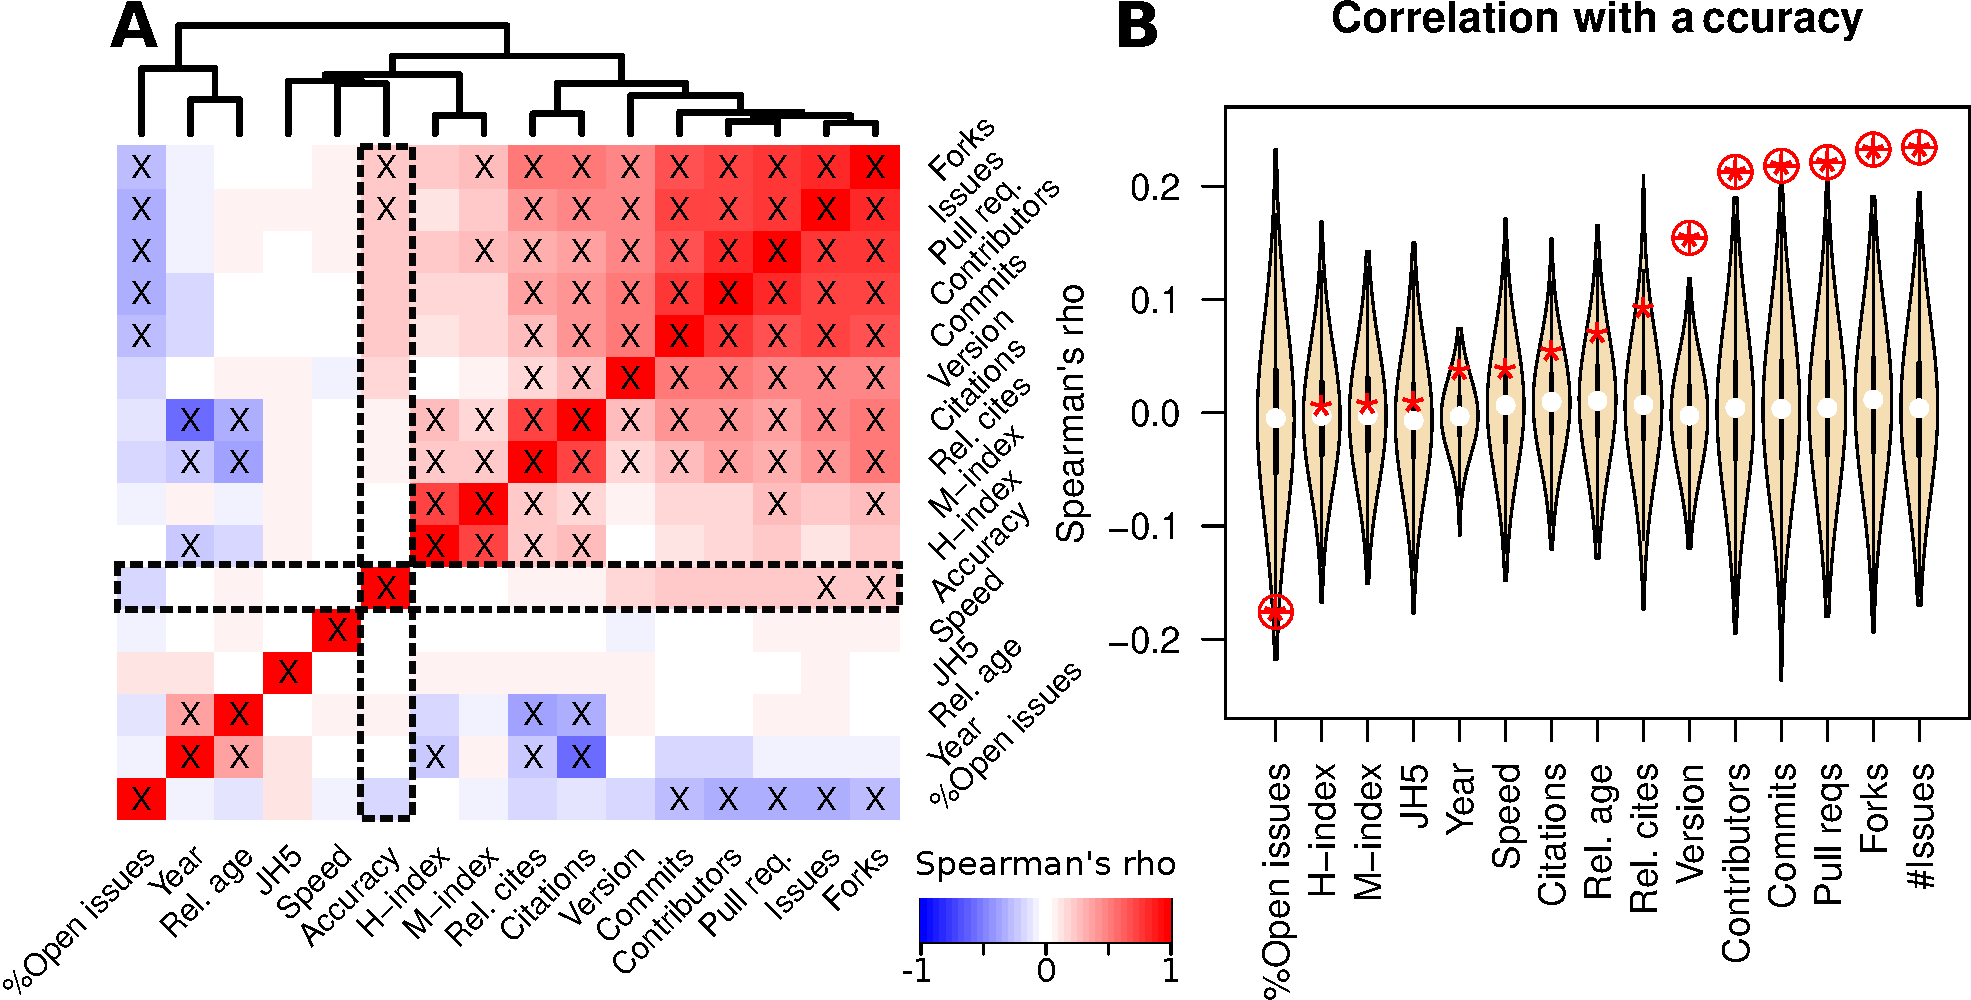
\includegraphics[width=0.9\textwidth]{figure1.pdf}
\caption{\textbf{A.} A heatmap indicating the relationships between
  different features of bioinformatic software tools. Spearman’s rho is used to
  infer correlations between metrics such as citations based metrics, the year and relative age of publication, 
  version number, GitHub derived activity measures, and 
  the mean
  relative speed and accuracy rankings. Red colours
  indicate a positive correlation, blue colours indicate a negative
  correlation. Correlations with an P-value less than 0.05 (corrected for multiple-testing using the Benjami-Hochberg method) are
  indicated with a `$\vartimes$' symbol. The correlations with accuracy are illustrated in
  more detail in \textbf{B}, the relationship between speed and
  accuracy is shown in more detail in \textbf{Figure 2}.
  %The
  %dendrogram was computed using the default ‘heatmap.2 function in R,
  %which computes a Euclidean distance matrix and a complete-linkage
  %hierarchical clustering.
  \textbf{B.} Violin plots of Spearman's correlations between permuted accuracy ranks and 
    different software tool features. 
    The unpermuted correlations are indicated with a red asterix.
    For each benchmark, 1,000 permuted sets of accuracy and speed ranks were generated, and the ranks were normalised to lie between 0 and 1 (see Methods for details).
  Circled asterixs are significant (empirical P-value $< 0.05$, corrected for multiple-testing using the Benjami-Hochberg method).}
\label{fig:allfactors}
\end{figure*}

For each of the publications describing these tools, we have (where
possible) collected the journal's H5-index (
%\href{https://scholar.google.co.nz/citations?view\_op=top\_venues\&hl=en}{
Google Scholar Metrics
%}
), the maximum H-index and
corresponding M-indices \cite{Hirsch2005-mt} for the corresponding
authors for each tool, and the number of times the publication(s)
associated with a tool has been cited using Google Scholar (data
collected over a 6 month period in late 2020). Note that citation metrics
are not static and will change over time. In addition, where possible we also extract the version number, the number
of commits, number of contributors
{\color{red} total number ``issues'', the proportion of issues that remain open, the number of pull requests, and the number of times the code was forked}
from public GitHub repositories.  

We have computed the Spearman’s correlation coefficient for each
pairwise combination of the mean normalised accuracy and speed ranks,
with the year published, mean relative age (compared to software in the
same benchmarks), journal H5 metrics, the total number of citations,
the relative number of citations (compared to software in the same
benchmarks) and the maximum H- and corresponding M-indices for the corresponding
authors, version number,
{\color{red}and the GitHub statistics commits, contributors, pull requests, issues, \% open issues and forks}.
The results are presented in Figure~\ref{fig:allfactors}A\&B and S5\&S6. We find
significant associations between most of the citation-based metrics
(journal H5, citations, relative citations, H-index and
M-index). There is also a negative correlation between the year of
publication, the relative age and many of the citation-based metrics.

Data on the number of updates to software tools from GitHub such as
the number of versions, commits and contributors was significantly
correlated with software accuracy (respective Spearman’s rhos =
{\color{black}0.15, 0.22, 0.21,} and respective Benjamini \& Hochberg
corrected P-values = {\color{black}0.029, 0.042, 0.063}),
Figure~\ref{fig:allfactors}B.  The significance of these features was
further confirmed with a permutation test
(Figure~\ref{fig:allfactors}B).  These features were not correlated
with speed however (see Figure~\ref{fig:allfactors}A {\color{red}\& Supplementary
Figures~S5 and~S6}%\ref{fig:S2}
).  We also found that
reputation metrics such as citations, author and journal H-indices,
and the age of tools were generally \textbf{not} correlated with
either tool accuracy or speed (Figure~\ref{fig:allfactors}A\&B).

%The strongest
%association was between accuracy and the relative
%number of citations (Spearman’s rho = {\color{black}0.092,
%P-value = 0.047}). But the effect size is only just over the
%significance threshold and may be the result of multiple-testing. 

%To further validate this result, we compute a correlation
%between speed and accuracy for each benchmark and used weighted sum
%Z-tests \cite{Zaykin2011-tj}. This also failed to identify a
%significant relationship (sum Z=-0.1, P-value=0.5).

In order to gain a deeper understanding of the distribution of
available bioinformatic software tools on a speed versus accuracy
landscape, we ran a permutation test. The ranks extracted
from each benchmark were randomly permuted, generating 1,000
randomized speed and accuracy ranks. In the cells of a $3\times3$
grid spanning the normalised speed and accuracy ranks we computed a
Z-score for the observed number of tools in a cell, compared to the
expected distributions generated by 1,000 randomized ranks. The results
of this are shown in Figure~\ref{fig:speedaccuracy}. We identified {\color{black}4}
of 9 bins where there was a significant excess or dearth of tools. For
example, there was an excess of ``slow and inaccurate'' software ({\color{black}Z=3.39,
P-value=$3.5\times 10^{-4}$}), with more moderate excess of ``slow and accurate'' and ``fast and accurate'' software (Z=2.49 \& 1.7, P=$6.3\times 10^{-3}$ \& 0.04 respectively). We find that only the ``fast and inaccurate'' extreme class is at approximately the
expected proportions based upon the permutation test (Figure 2B).

% binom.test(sigCount,gridRes^2, p = 0.05)

\begin{figure*}[htb!]
%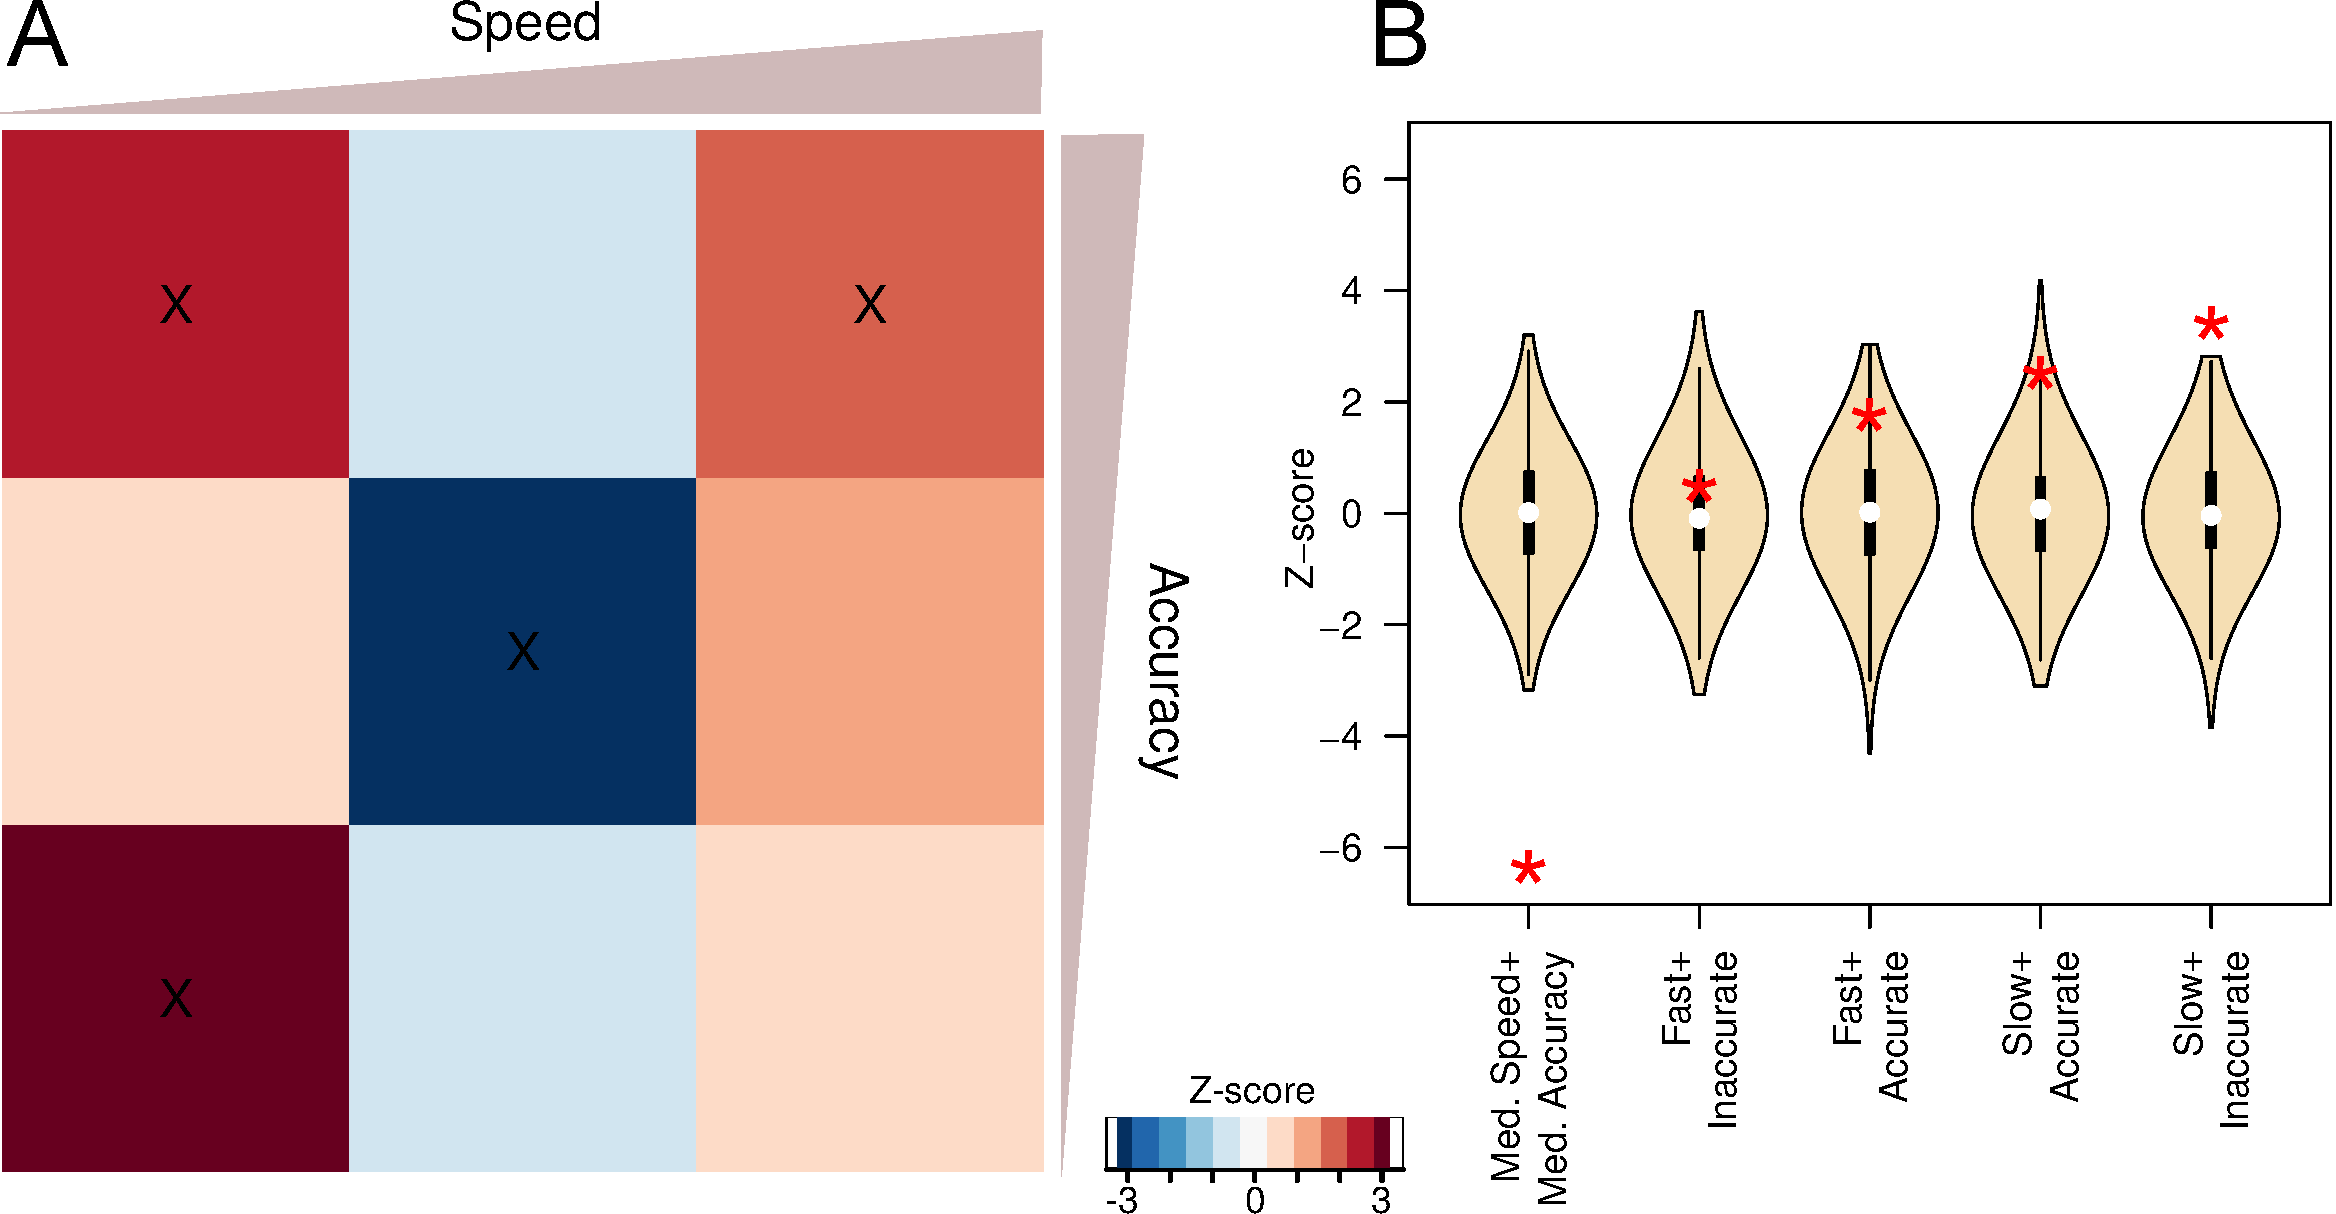
\includegraphics[scale=0.55]{figure2.pdf}
\centering
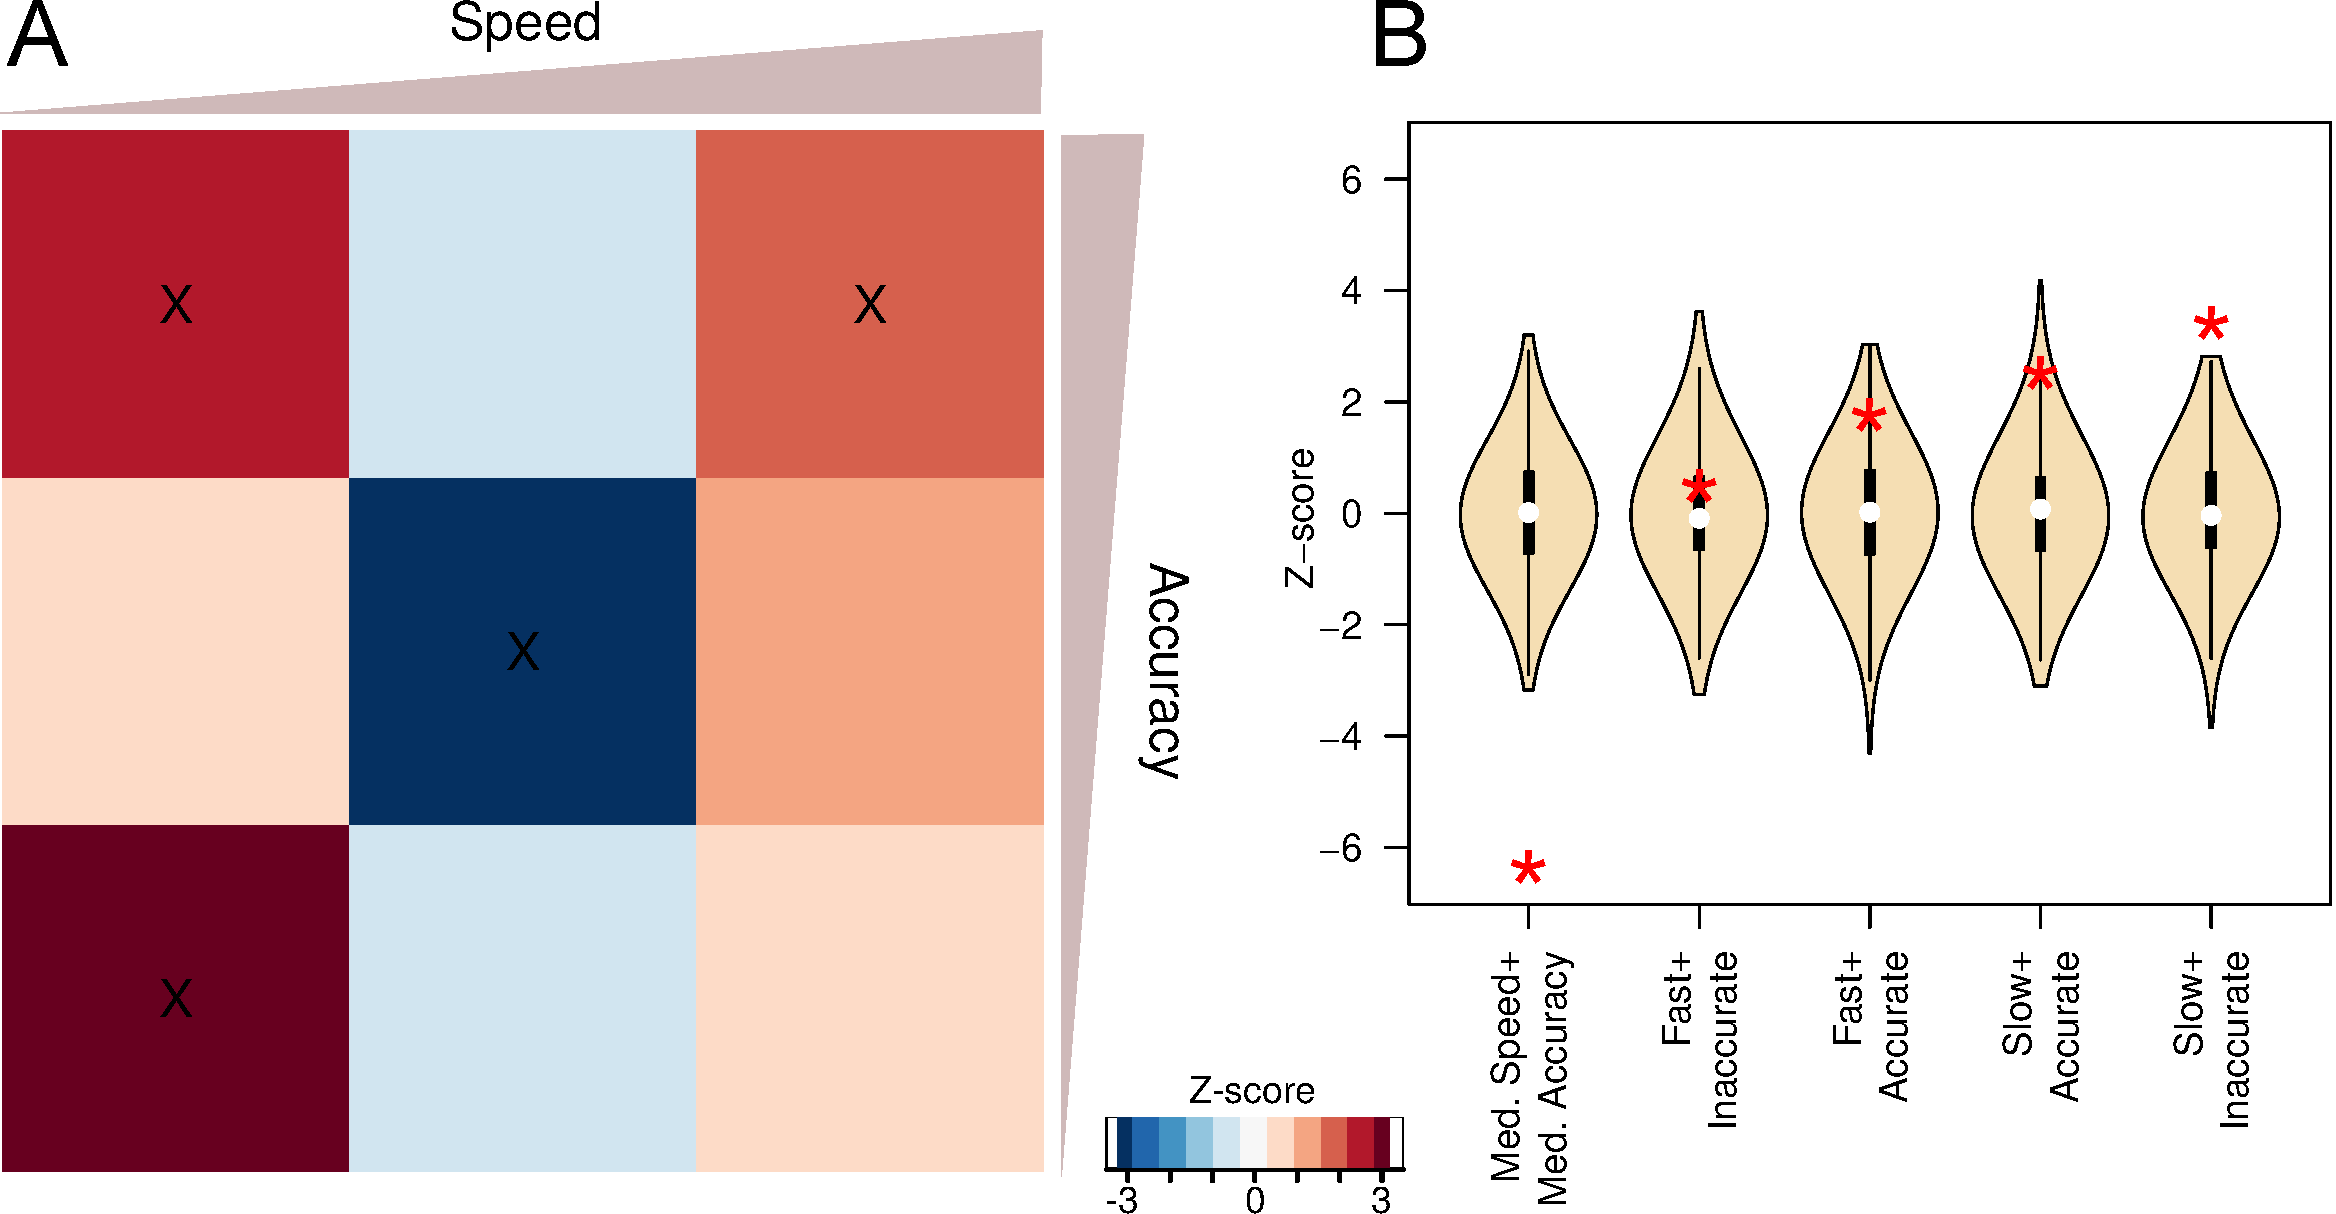
\includegraphics[width=0.95\textwidth]{figure2.pdf}
\caption{\textbf{A.} A heatmap indicating the relative paucity or abundance of
  software in the range of possible accuracy and speed rankings. Redder
  colours indicate an abundance of software tools in an accuracy and
  speed category, while bluer colours indicate scarcity of software in
  an accuracy and speed category. The abundance is quantified using a
  Z-score computation for each bin, this is derived from 1,000 random
  permutations of speed and accuracy ranks from each
  benchmark. Mean normalised ranks of accuracy and speed have been
  binned into 9 classes (a $3\times 3$ grid) that range from
  comparatively slow and inaccurate to comparatively
  fast and accurate. Z-scores with a P-value less than 0.05 are indicated
  with a ‘$\vartimes$’. \textbf{B.} The z-score distributions from the permutation tests (indicated with the wheat coloured violin plots) compared to 
  the z-score for the observed values for each of the corner and middle square of the heatmap.}
\label{fig:speedaccuracy}
\end{figure*}

The largest difference between the observed and expected software ranks is the reduction in the number of software tools that are
classed as intermediate in terms of both speed and accuracy based on
permutation tests (see Methods for details, Figure~\ref{fig:speedaccuracy}). The middle cell
of Figure 2A and left-most violin plot of Figure 2B highlight this extreme, (Z=-6.38,
P-value=$9.0\times 10^{-11}$). 

\section*{Conclusion}

We have gathered data on the relative speeds and accuracies of
{\color{black}\numTools~} bioinformatic tools from
{\color{black}\numBenchmarkPubs} benchmarks published between
2005 and 2020. Our results provide significant support for the suggestion that there are major benefits to
the long-term support of software development \cite{siepel2019challenges}. The
finding of a strong relationship between the number of commits and code contributors to
GitHub (i.e. software updates) and accuracy, highlights the benefits of
long-term or at least intensive development.

Our study finds little evidence to support that impact-based metrics
have any relationship with software quality, which is unfortunate, as these
are frequently cited reasons for selecting software tools
\cite{Loman2015-bw}. This implies that high citation
rates for bioinformatic software
\cite{Perez-Iratxeta2007-lv,Van_Noorden2014-kc,Wren2016-xy} is more a
reflection of other factors such as user-friendliness or the Matthew Effect
\cite{Lariviere2010-kx,Merton1968-cb} other than accuracy.

We found the lack of a correlation between software speed and accuracy
surprising.  The slower software tools are overrepresented at both
high and low levels of accuracy (Figure~\ref{fig:speedaccuracy}).
In addition, there is an large under-representation of software that has
intermediate levels of both accuracy and speed. A possible explanation
for this is that bioinformatic software tools are bound by a form of
publication-bias \cite{Boulesteix2015-am,Nissen:2016}. That is, the
probability that a study being published is influenced by the results
it contains \cite{sterling1995publication}. The community of
developers, reviewers and editors may be unwilling to publish software
that is not highly ranked on speed or accuracy. If correct, this may
have unfortunate consequences as these tools may {\color{red}nevertheless} have further uses.
%We also found that slow and inaccurate
%software is generally published earlier than fast and accurate tools
%{\color{black}(P=0.007, one-tailed Wilcoxon test)}, therefore
%comparisons with existing software were not required to publish the slow and
%inaccurate tools.

%% A
%% gedankenexperiment may be sufficient to show that slow software is
%% less thoroughly tested than fast software. This is because typical
%% academic software development is an iterative process, where tools are
%% refined by successive rounds of coding, testing and evaluation
%% \cite{Wilson2006-ih}. We can assume that similar time-spans are spent
%% on most projects, for example, the span of a PhD degree or
%% Postdoctoral Fellowship.  As a consequence, slow software may undergo
%% fewer development cycles than faster tools.

While we have taken pains to mitigate many issues with our analysis, nevertheless 
some limitations remain. For example, it has proven difficult to verify if the gap in medium accuracy 
and medium speed software is genuinely the result of publication bias, or due to additional factors that we have 
not taken in to account. In addition, all of the features we have used here are moving targets. For example, as software 
tools are refined, their relative accuracies and speeds will change, the citation metrics, ages, and version control 
derived measures also change over time. Here we report a snapshot of values from 2020.  The benchmarks themselves may 
also introduce biases into the study. For example, there are issues with a potential lack of independence between benchmarks 
(e.g., shared datasets, metrics and tools), there are heterogeneous measures of accuracy and speed and often unclear 
processes for including different tools. 

%{\bf DESCRIBE STUDY LIMITATIONS... 
%\begin{itemize}
%    \item Difficult to test publication biases
%    \item Heterogeneous measures of accuracy between benchmarks  
%    \item possible lack of independence between different benchmarks 
%    \item Non-uniform inclusion of tools in different benchmarks -- some tools ranked many times (e.g. velvet and soap assemblers ranked 26 different times)
%    \item How to deal with inconsistently reported versioning of software? 
%    \item Metrics and tools performance are all moving targets, only a snap shot is used here  
%\end{itemize}
%}


We propose that the full spectrum of software tool accuracies and
speeds serves a useful purpose to the research community. Like negative
results, if honestly reported this information, illustrates to the research community
that certain approaches are not practical research avenues
\cite{fanelli2012negative}. % Ioannidis2005-xh,Workman1999-au,Rivas2000-fb}.
The current
practices of publishers, editors, reviewers and authors of software
tools therefore may be depriving our community of tools for building effective
and productive workflows.

The most reliable way to identify accurate software tools is through neutral
software benchmarks \cite{Boulesteix2013-vb}. We are hopeful that
this, along with steps to reduce the publication-bias we have
described, will reduce the over-optimistic and misleading reporting of
tool accuracy \cite{Boulesteix2010-te,Jelizarow2010-zf,Norel2011-cq}.


\section*{Methods}
In order to evaluate predictors of computational biology software
accuracy, we mined the published literature, extracted data from
articles, connected these with bibliometric databases, and tested for
correlates with accuracy. We outline these steps in further detail
below.

\textbf{Criteria for inclusion:} We are interested in using
computational biology benchmarks that satisfy Boulesteix’s
(ALB) three criteria for a ``neutral comparison study''
\cite{Boulesteix2013-vb}. Firstly, the main focus of the article is
the comparison and \textbf{not} the introduction of a new
tool {{\color{red}as these can be biased} \cite{Buchka:2021a}. Secondly, the authors should be reasonably neutral, which means
that the authors should not generally have been involved in the
development of the tools included in the benchmark. Thirdly, the test
data and evaluation criteria should be sensible. This means that the
test data should be independent of data that tools have been trained
upon, and that the evaluation measures appropriately quantify correct
and incorrect predictions.

\textbf{Literature mining:} We identified an initial list of 10 benchmark
articles that satisfy the ALB-criteria. These were identified based
upon previous knowledge of published articles and were supplemented
with several literature searches (e.g., [``benchmark'' AND ``cputime''] was
used to query both GoogleScholar and Pubmed
\cite{Sayers2010-vm,McEntyre2001-fl}). We used these articles to seed
a machine-learning approach for identifying further candidate articles
and to identify new search terms to include.

For our machine-learning-based literature screening, we computed a
score, $s(a)$, for each article that tells us the likelihood that it
is a benchmark. In brief, our approaches uses 3 stages:
\begin{enumerate}
\item Remove high frequency words from the title and abstract of candidate articles (e.g. ‘the’, ‘and’, ‘of’, ‘to’, ‘a’, …) 
\item Compute a log-odds score for the remaining words 
\item Use a sum of log-odds scores to give a total score for candidate articles
\end{enumerate}
For stage 1, we identified a list of high frequency (e.g. $f$(word) $>$
$1/10,000$) words by pooling the content of two control texts
\cite{Carroll1865-hk,Tolkien1937-ke}.

For stage 2, in order to compute a log-odds score for bioinformatic
words, we computed the frequency of words that were not removed by our
high frequency filter in two different groups of articles:
bioinformatics-background and bioinformatics-benchmark articles. The
text from bioinformatics-background articles were drawn from the
bioinformatics literature, but these were not necessarily associated
with benchmark studies. For background text we used Pubmed
(\cite{Sayers2010-vm,McEntyre2001-fl} to select 8,908 articles that
contained the word “bioinformatics” in the title or abstract and were
published between 2013 and 2015. We computed frequencies for each word
by combining text from titles and abstracts for the background and
training articles. A log-odds score was computed for each word using
the following formula:
%\todo{Word is denoted $w$ on the left and $word$ on the right.}

\[lo(word)=\log_2\frac{f_{tr}(word)+\delta}{f_{bg}(word)+\delta}\] 

Where
$\delta$
was a pseudo-count added for each word ($\delta = 10^{-5}$, by default),
$f_{bg}(word)$ and $f_{tr}(word)$ were the frequencies of a $word$ in
the background and training datasets respectively. Word frequencies
were computed by counting the number of times a word appears in the
pool of titles and abstracts, the counts were normalised by the total
number of words in each set.

Thirdly, we also collected a group of candidate benchmark articles by
mining Pubmed for articles that were likely to be benchmarks of
bioinformatic software, these match the terms: “((bioinformatics)
AND (algorithms OR programs OR software)) AND (accuracy OR assessment
OR benchmark OR comparison OR performance) AND (speed OR
time)”. Further terms used in this search were progressively added as
relevant enriched terms were identified in later iterations. The final
query is given in \textbf{supplementary materials}.

A score is computed for each candidate article by summing the log-odds
scores for the words in title and abstract,
i.e. $s(a)=\sum_i^Nlo(w_i)$. The high scoring candidate articles are
then manually evaluated against the ALB-criteria. Accuracy and speed
ranks were extracted from the articles that met the criteria, and
these were added to the set of training articles. The evaluated
candidate articles that did not meet the ALB-criteria were incorporated
into the set of background articles. This process was iterated and resulted in the identification of
{\color{black}\numBenchmarkPubs} benchmark articles,
containing {\color{black}\numBenchmarks} different benchmarks. Together these
ranked {\color{black}\numTools~} distinct software packages.

There is a potential for bias to have been introduced into this
dataset. Some possible forms of bias include converging on a niche
group of benchmark studies due to the literature mining technique that
we have used. A further possibility is that benchmark studies
themselves are biased, either including very high performing or very
low performing software tools. To address each of these concerns we
have attempted to be as comprehensive as possible in terms of
benchmark inclusion, as well as including comprehensive benchmarks (i.e.,
studies that include all available software tools that
address a specific biological problem).

\textbf{Data extraction and processing:} for each article that met the
ALB-criteria and contained data on both the accuracy and speed from
their tests, we extracted ranks for each tool. {\color{red}Until published datasets are made available in consistent, machine-readable formats this step is necessarily a manual process -- ranks were extracted from a mixture of manuscript figures, tables and supplementary materials, each data source is documented in Supplementary Table 1. In addition, a variety of accuracy metrics are reported e.g. ``accuracy'', ``AUROC'', ``F-measure'', ``Gain'', ``MCC'', ``N50'', ``PPV'', ``precision'', ``RMSD'', ``sensitivity'', ``TPR'', ``tree error'', etc. Our analysis makes the necessarily pragmatic assumption that highly ranked tools on one accuracy metric will also be highly ranked on other accuracy metrics.}
Many articles contained
multiple benchmarks, in these cases we recorded ranks from each of these, the
provenance of which is stored with the accuracy metric and raw speed
and accuracy rank data for each tool {\color{red}(Supplementary Table 1)}. In line with rank-based
statistics, the cases where tools were tied were resolved by using a
midpoint rank (e.g., if tools ranked 3 and 4 are tied, the rank 3.5 was used)
\cite{Mann1947-re}. Each rank extraction was independently verified by
at least one other co-author to ensure both the provenance of the data
could be established and that the ranks were correct. The ranks for
each benchmark were then normalised to lie between 0 and 1 using the
formula $1-\frac{r-1}{n-1}$ where ‘$r$’ is a tool’s rank and ‘$n$’ is the
number of tools in the benchmark. For tools that were benchmarked
multiple times with multiple metrics (e.g., BWA was evaluated in 6
different articles
\cite{Bao2011-lv,Caboche2014-lj,Hatem2013-cs,Schbath2012-ob,Ruffalo2011-rl,Holtgrewe2011-fd})
a mean normalised rank was used to summarise the accuracy and speed performance. 
Or, more formally:
 
\begin{equation*}
\begin{split}
accuracy =& \sum_{i=1..N} 1-\frac{r^{accuracy}_i-1}{n_i-1}, \\
speed    =& \sum_{i=1..N} 1-\frac{r^{speed   }_i-1}{n_i-1}
\end{split}
\end{equation*}
 
For each tool we identified the corresponding publications in
GoogleScholar; the total number of citations was recorded, the
corresponding authors were also identified, and if they had public
GoogleScholar profiles, we extracted their H-index and calculated a
M-index ($\frac{H-index}{y}$) where ‘$y$’ is the number of years since
their first publication. The journal quality was estimated using the H5-index
from GoogleScholar Metrics. 

The year of publication was also recorded for each
tool. “Relative age” and “relative citations” were also computed for
each tool. For each benchmark, software was ranked by year of first
publication (or number of citations), ranks were assigned and then
normalised as described above. Tools ranked in multiple evaluations
were then assigned a mean value for “relative age” and “relative
citations”.

The papers describing tools were checked for information on version numbers and links to GitHub. 
Google was also employed to identify GitHub repositories. When a repository was matched with a tool, the number of ``commits'' and number of ``contributors'' was collected, when details of version numbers were provided, these were also harvested. 
Version numbers are inconsistently used between groups, and may begin at either 0 or 1. To counter this issue we have added `1' to all versions less than `1', for example, version 0.31 become 1.31. In addition, multiple point releases may be used e.g. `version 5.2.6', these have been mapped to the nearest decimal value `5.26'.

\textbf{Statistical analysis:} For each tool we manually collected up to 12 different
statistics from GoogleScholar, GitHub and directly from literature describing tools 
(1. corresponding author’s H-index, 
2. corresponding author’s M-index, 
3. journal H5 index, 
4. normalised accuracy rank, 
5. normalised speed rank, 
6. number of citations, 
7. relative age, 
8. relative number of citations, 
9. year first published, 
10. version
11. number of commits to GitHub,
12. number of contributors to GitHub). 
These were evaluated in a pairwise fashion to
produce Figure~\ref{fig:allfactors} A\&B, the R code used to generate these is
given in a GitHub repository (linked below).

%The linear models that we used to test for relationships between
%speed, accuracy and the above measures are:
%
%\begin{equation*}
%\begin{split}
%accuracy=& c_0+c_1\times speed+c_2\times JIF+c_3\times H5+\\
%& c_4\times citations+c_5\times Hindex+\\
%& c_6\times Mindex+c_7\times relativeAge+\\
%& c_8\times relativeCitations
%\end{split}
%\end{equation*}
%
%\begin{equation*}
%\begin{split}
%speed=& c_0+c_{1}\times accuracy+c_{2}\times JIF+c_{3}\times H5+\\
%& c_{4}\times citations+c_{5}\times Hindex+\\
%& c_{6}\times Mindex+c_{7}\times relativeAge+\\
%& c_{8}\times relativeCitations
%\end{split}
%\end{equation*}

For each benchmark of three or more tools, we extracted the published
accuracy and speed ranks. In order to identify whether there was an
enrichment of certain accuracy and speed pairings we constructed a
permutation test. The individual accuracy and speed ranks were
reassigned to tools in a random fashion and each new accuracy and
speed rank pairing was recorded. For each benchmark this procedure was
repeated 1,000 times. These permuted rankings were normalised and
compared to the real rankings to produce the ‘$\vartimes$’ points in
Figure~\ref{fig:allfactors}B and the heatmap and histograms in
Figure~\ref{fig:speedaccuracy}. The heatmap in
Figure~\ref{fig:speedaccuracy} is based upon Z-scores
($Z=\frac{x-\bar{x}}{s}$). For each cell in a $3\times 3$ grid
a Z-score (and corresponding P-value is computed, either with the `pnorm' distribution function in R (Figure 2A) or empirically (Figure 2B)) is computed to illustrate the abundance or lack of tools in
a cell relative to the permuted data.


\begin{backmatter}

\section*{Acknowledgements}
The authors acknowledge the valued contribution of invaluable
discussions with Anne-Laure Boulesteix, Shinichi Nakagawa, Suetonia
Palmer and Jason Tylianakis. Murray Cox, Raquel
Norel, Alexandros Stamatakis, Jens Stoye, Tandy Warnow, and 
Luis Pedro Coelho provided
valuable feedback on drafts of the manuscript.

This work was largely conducted on the traditional territory of K\=ai Tahu.

\section*{Funding}
PPG is supported by a Rutherford Discovery Fellowship,
administered by the Royal Society Te Ap\=arangi, 
PPG, AG and MAB acknowledge support from a Data Science Programmes grant
(UOAX1932).

\section*{Availability of data and materials}
%\section*{Data availability}
Raw datasets, software and documents are available under a CC-BY license:\\
%\fussy
%\url{https://docs.google.com/spreadsheets/d/14xIY2PHNvxmV9MQLpbzSfFkuy1RlzDHbBOCZLJKcGu8/edit?usp=sharing}\\
%and here:\\
%\fussy
%\url{https://dx.doi.org/10.6084/m9.figshare.4299320.v1}\\
%\sloppy
%Additional documentation, code, figures and raw data is available here:\\
\fussy
\url{https://github.com/Gardner-BinfLab/speed-vs-accuracy-meta-analysis}
\sloppy

\section*{Competing interests}
The authors declare that they have no competing interests.


%----------------------------------------------------------------------------------------
%	REFERENCE LIST
%----------------------------------------------------------------------------------------
%\bibliographystyle{unsrt}
\bibliographystyle{bmc-mathphys}
\bibliography{references.bib}

\end{backmatter}
\end{document}
